\documentclass[10pt,a4paper]{article}
\usepackage[utf8]{inputenc}
\usepackage[magyar]{babel}
\usepackage{amsmath}
\usepackage{multicol}
\usepackage{amsfonts}
\usepackage{amssymb}
\usepackage{hyperref}
\hypersetup{
	colorlinks=true,
	linkcolor=black,
	filecolor=magenta,      
	urlcolor=blue,
}
\usepackage{graphicx}
\usepackage{geometry}
\geometry{a4paper,
	total={210mm,297mm},
	left=2cm,
	right=2cm,
	top=20mm,
	bottom=20mm,
}
\title{Kommunikációs hálózatok 2 jegyzet}
\author{Lant Gábor}

\begin{document}
\maketitle
\noindent Source: \url{https://github.com/lantgabor/KH2-jegyzet}
\tableofcontents
\section{Előszó}
Ez a \textbf{nem hivatalos} jegyzet a 2019-es Kommunikációs hálozatok 2 (VITMAB01) tárgyhoz készült. A jegyzet semmiképpen nem helyettesíti az előadásokon való részvételt, nem tartalmazza a jegyzetben "nem vizsgaanyag"-ként megjelölt részeket, illetve lehetnek benne hiányosságok vagy hibák. A zh-ra való felkészülés segítésére készítettem. Ezért örülnék minden pull requestnek és issuenak.
\newpage
\section{Beszédátvitel, telefonrendszerek}
\begin{itemize}
\item Végberendezés/Endpoint: Klasszikusan: Telefonkészülékek.\\
\item Kapcsolóközpontok: Egymással hierarchikusan összekötve\\
\item Átviteli utak: Előfizető $\leftrightarrow $ Központ, local loop/helyi hurok (rézpár)\\
központok: Trönk (trunk) pl. koax, rádiós,fényszál
\item Next Generation Networks: 2004 körüli koncepció,. Ötlet: egyetlen, csomagkapcsolt (IP) gerinchálózat + extra szolgáltatások: TV,telefon,ADSL
\begin{center}
	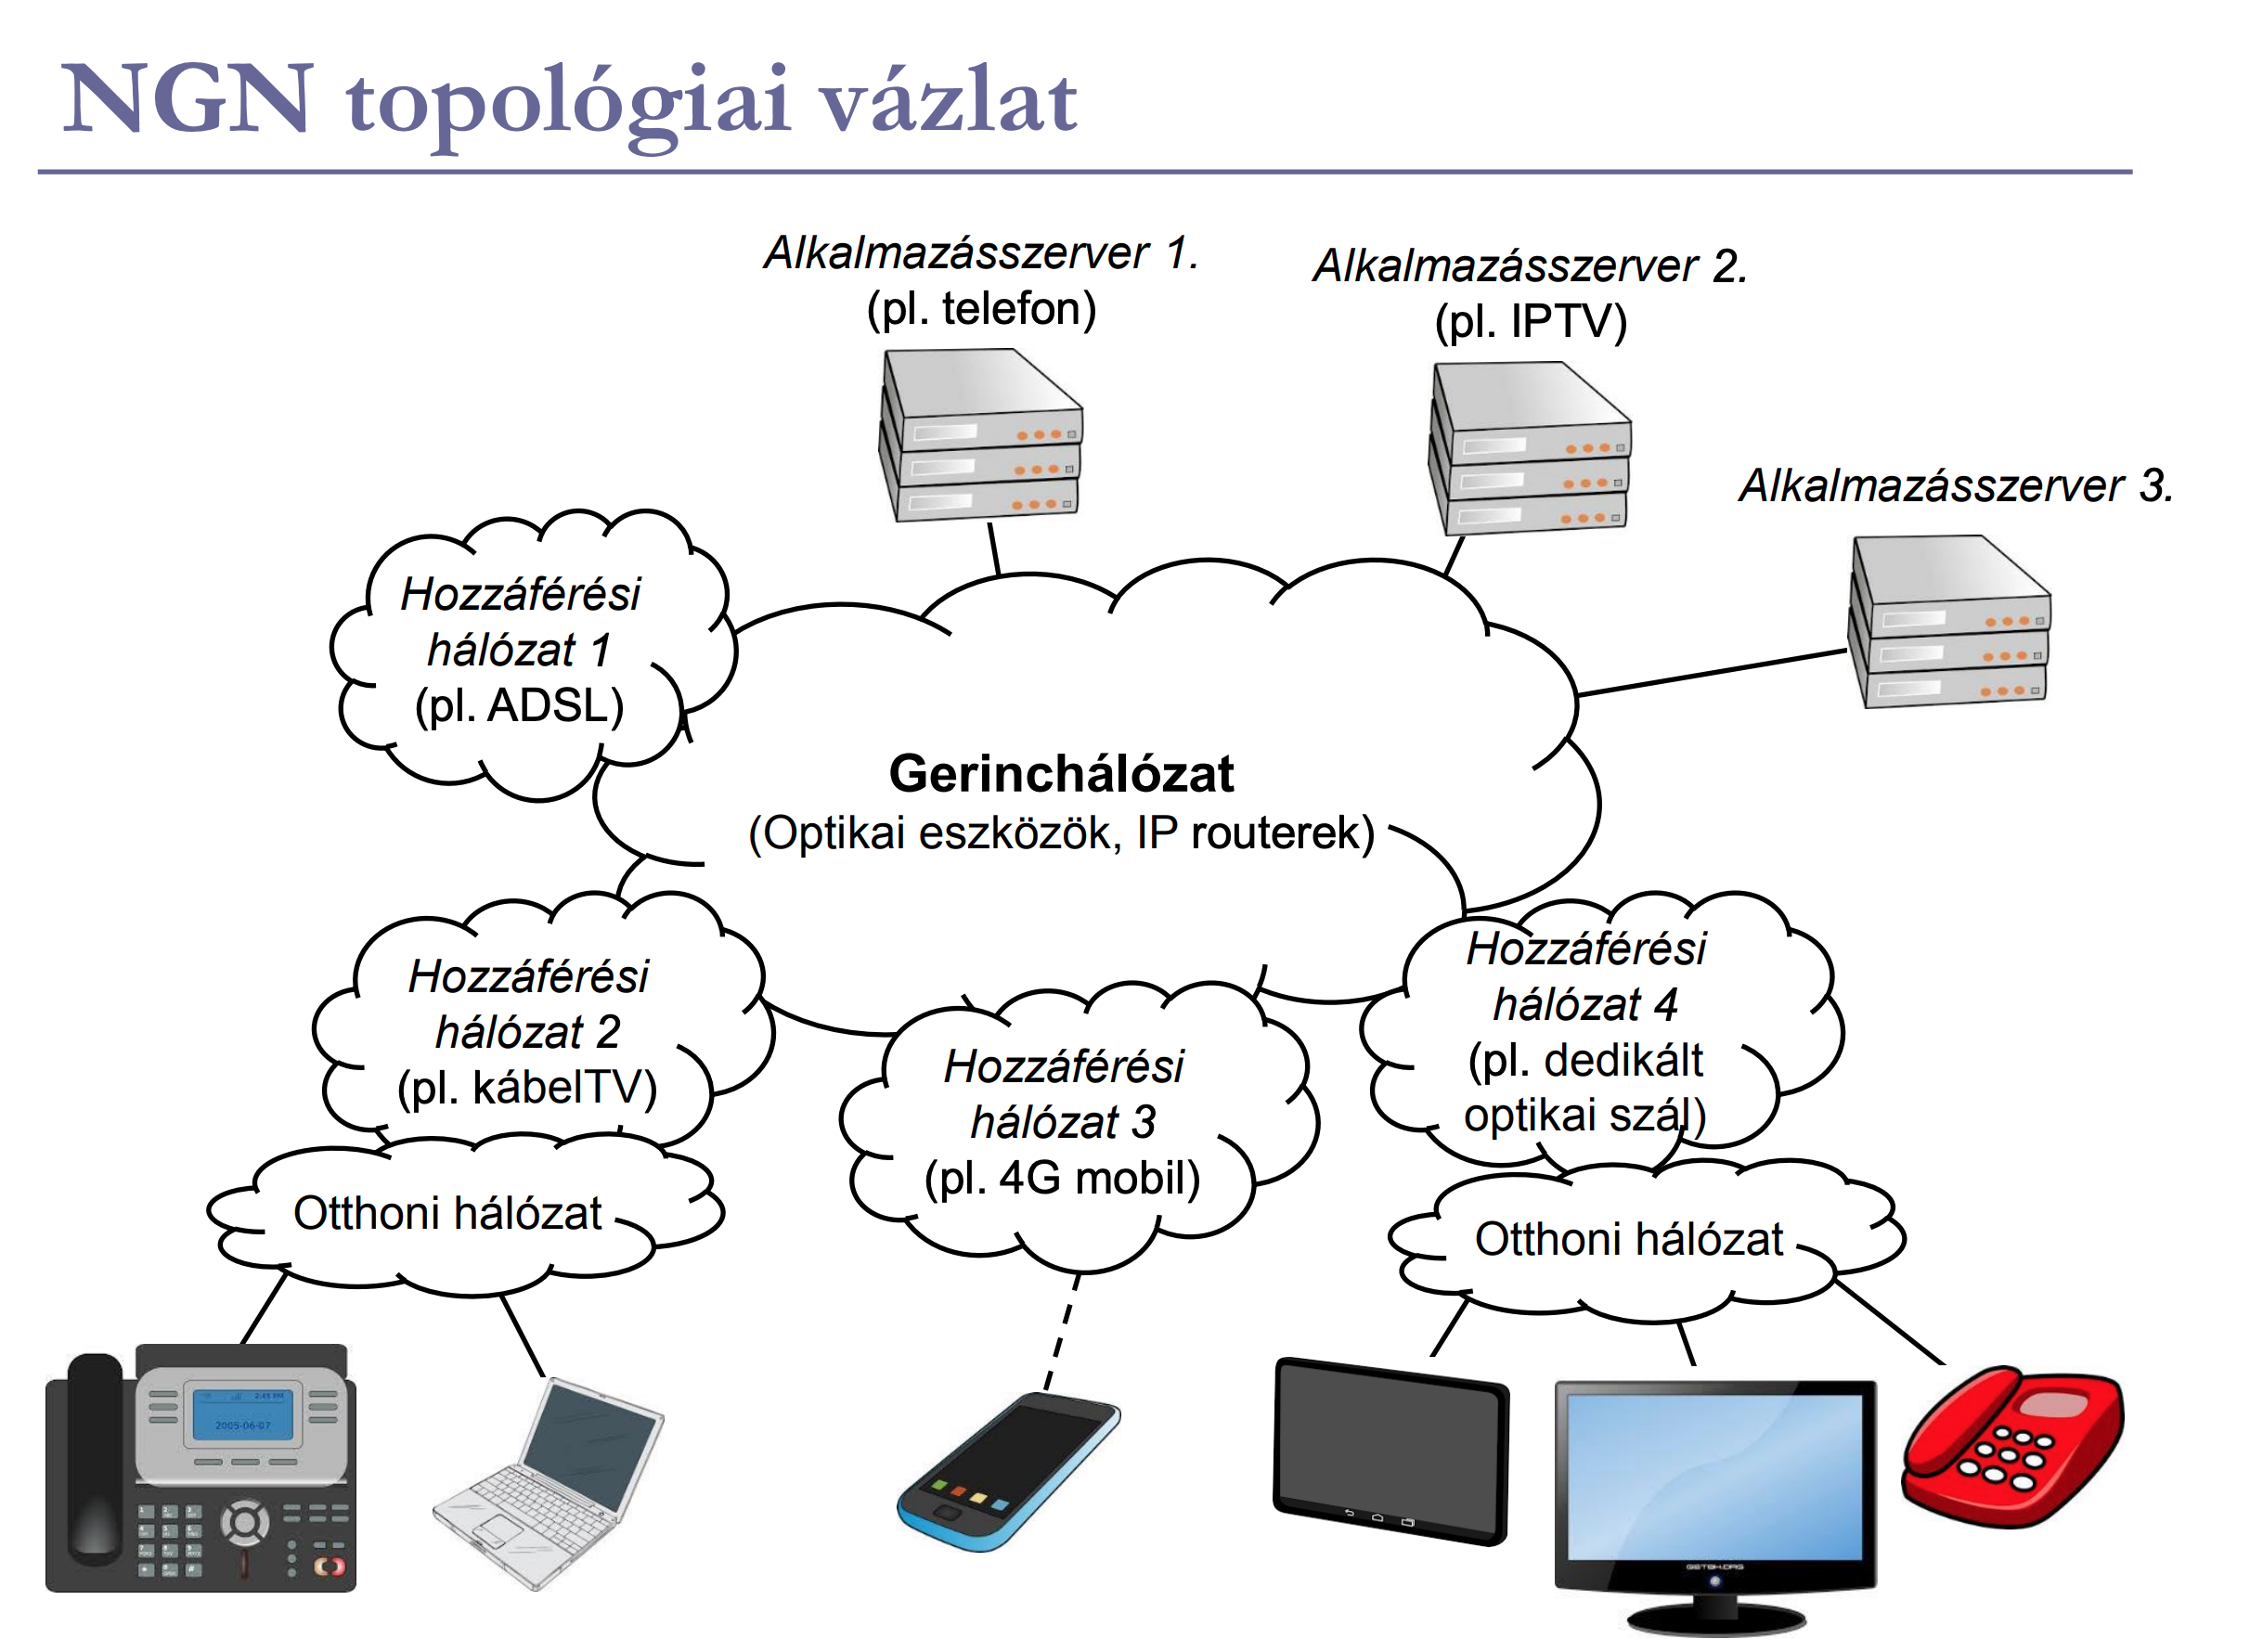
\includegraphics[width=0.9\linewidth]{src/NNG}
\end{center}
\end{itemize}
\fbox{\begin{minipage}[\textwidth]{0.9\textwidth}
	Dense Wavelenght Multiplexing $\rightarrow$ MPLS $\rightarrow$ Aggregációs hálózat $\rightarrow$ (xDSL, Optikai hozzáférés, KábelTV, Mobil, stb.) $\rightarrow$ Szélessávú hozzáférési hálózat $\rightarrow$ Felhasználói végberendezés.
\end{minipage}}

\section{Számozás}
Számítógép-hálózatoknál címzésnek hívják (Numbering vs.
addressing)\\
\begin{tabular}{|c|c|}
	\hline 
	 1  &Észak-Amerika\\ 
	\hline 
	2 &Afrika+Grönland  \\ 
	\hline 
	3,4&Európa  \\ 
	\hline 
	5&Közép- és Dél-Amerika  \\ 
	\hline 
	6& Ausztrália és Óceánia \\ 
	\hline 
	7&Oroszország, Kazahsztán \\ 
	\hline 
	8&  Távol-Kelet (+Inmarsat,
	Nemzetk. zöld szám: 800)\\ 
	\hline 
	9& Közel- és Közép-Kelet\\ 
	\hline 
\end{tabular} 
\begin{itemize}
	\item Országon belül: belföldi rendeltetési szám + előfizetői
	szám
	\item Belföldi rendeltetési szám:
	Körzetszám, pl.: 33: Esztergom és környéke (földrajzi számok)
	Hálózatkijelölő szám, pl: 20: Telenor
	Szolgáltatáskijelölő szám, pl: 90: emeltdíjas
	\item Fontos: a telefonszámok mindig prefix kódok
	azaz nem lehet egyik szám egy másik folytatása
	\item Nyílt számozási rendszer: Nem kell mindig a belföldi rendeltetési számot tárcsázni
	\item Zárt számozási rendszer: Mindig kell a belföldi rendeltetési szám, Nem kell viszont a belföldi előtét (0, vagy Magyarországon 06)
	\item 2010-től már mindig kell, mobilszámmező lezárása.
\end{itemize}
\section{Analóg beszédátvitel}
\begin{itemize}
	\item\textbf{ Cél: érthető beszéd átvitele. Régen FreqDivMult. Most: TimeDivMult.}\\
Jó hangminőség: \textbf{0.3 -- 3.4 kHz} $\rightarrow$ 3,1 kHz + védősávok = \textbf{4 kHz széles lesz egy beszédcsatorna}
\item Digitális technika:\begin{itemize}
	\item kapcsolás megvalósítható mozgó alkatrészek nélkül
\item magasabb fokú hálózati intelligencia valósítható meg
\item sokkal kifinomultabb jelzésátvitel lehetséges
\item adat és beszédjelek egységesen kezelhetőek
\end{itemize}
\item beszéddigitalizáló (kódoló-dekódoló: kodek)
\end{itemize}
\section{PCM (Pulse Code Modulation, Impulzuskód moduláció)}
\begin{itemize}
	\item Adott egy „jel”: feszültség-idő függvény
	\item \textbf{A-D átalakítás lépései}
\begin{itemize}
	\item sávszűrés
	\item mintavétel
	\item kvantálás
	\item kódolás
\end{itemize}
	\item \textbf{D-A átalakítás lépései}
\begin{itemize}
	\item D-A átalakítás a kvantálás inverz karakterisztikjáváal
	\item sávszűrés (simítás)
\end{itemize}
\item \textbf{Mintavételezés}
\begin{itemize}
	\item Van olyan, hogy elég minta a tökéletes
	visszaállításhoz?
	\item \textbf{Nyquist-Shannon mintavételi tétele:}
	\item Igen! A jel max. \textbf{frekvenciájának duplája} elég
	mintavételi frekvencia
\end{itemize}
\item \textbf{Kvantálás}
\begin{itemize}
	\item Van olyan, hogy elég kvantálási szint a tökéletes
	visszaállításhoz? Nincs :(
	\item Mindig marad hiba: a \textbf{kvantálási torzítás}
	\item kevésbé precízen: „kvantálási zaj”
	\item Megoldás: \textbf{nem egyenletes kvantálás}
	\item logaritmikus karakterisztikával (az emberi fül is ilyen)
	\item USA: $\neq$ törvényű kvantáló \textbf{($\mu$-law)}
	\item Európa: A törvényű kvantáló \textbf{(A-law)}
	\item hasonló, de nem kompatibilis, átkódolás kell
\end{itemize}
\item Számolás: 8000 $\frac{minta}{sec} \star$ 8 $\frac{bit}{minta}$ = 64 $kb/s$
\item \textbf{Auido CD-n is PCM-et használnak}
\subitem Mintavételezés: 44.100 Hz
\subitem Kvantálás: 16 bit (65.536 szint)
\subitem Sztereó: 2 független csatorna
\subitem Bitsebesség: $44.100 minta/s/csatorna * 16 bit/minta * 2 csatorna = 1.411.200 bit/s \approx 1,4 Mb/s \approx 176,4 kB/s$
\end{itemize}
\section{Beszédkódolók (Kodek, Codec)}
\begin{itemize}
	\item Ugyanaz a kódoló mindkét oldalon, vagy hálózaton belüli konverzió
	\item bitsebesség: \textbf{2,4 -- 64 kb/s}
	\item \textbf{MOS (Mean Opinion Score, átlagolt véleménypontok)}
	\item \textbf{kódolási késleltetés:} minél nagyobb időszeletet dolgozunk fel egyszerre, annál jobban
	tömöríthetünk – nagyobb késleltetés árán: 0,125 – 80 ms
	\item \textbf{komplexitás}
\end{itemize}
\subsection{Kodek jellemzők}
\begin{itemize}
	\item \textbf{robosztusság:} hiba esetén nincs idő újraadásra, hibajavító kódolás, FEC (Forward Error Correction, előremenő hibajavítás)
	\item \textbf{tandemezhetőség és átkódolhatóság} (egymás után csatolás)
	\item \textbf{átlátszóság:} Hang (300-3400 Hz között), de nem beszédhang átvihető-e?
	\subitem Pl. a DTMF (Dual Tone MultiFrequency, kéthangú többfrekvenciás
	jelzésátviteli rendszer)
	\item \textbf{adaptivitás}
	\subitem terhelés esetén kisebb jelsebesség
	\subitem de: a hálózat nehezebben tervezhető
\end{itemize}
\subsection{Kódoló típusok}
\begin{itemize}
	\item  \textbf{Hullámforma kódoló}
\begin{itemize}
	\item analóg jel alakjának a megőrzése
	\item jó minőség
	\item nagy bitsebesség (ez hátrány, nem előny! :) )
	\item átlátszóság
\end{itemize}
	\item \textbf{Vokóder}
\begin{itemize}
	\item adó oldalon: beszédből jellemző paraméterek kiszűrése
	\item vevő oldalon: ezek alapján beszédszintetizálás
	\item kis sebesség
	\item eredetire nem nagyon hasonlító hang
\end{itemize}
	\item \textbf{Hibrid kódoló}
	\begin{itemize}
	\item előbbiek keveréke
\end{itemize}
\item\textbf{ AMR-WB:} Adaptive Multirate, Wideband \textbf{(HD hang)}
\begin{itemize}
\item bő 10 éves szabvány, az utóbbi időben kezdték bevezetni
\subitem mindhárom mobilszolgáltatónál
\subitem egy hálózaton belül csak
\subitem kizárólag 3G mobilhálózaton
\item Szélesebb spektrum, 16 kHz mintavételezés + más javítások a
kódolón: nagyobb adatsebesség, jobb minőség
\end{itemize}
\end{itemize}
\begin{tabular}{|c|c|c|}
	\hline 
	Kódoló neve & Fő
	alkalmazás & Adatsebesség
	(kb/s) \\ 
	\hline 
	PCM & vezetékes
	távb. h & 64 \\ 
	\hline 
	(GSM) FR & GSM & 13 \\ 
	\hline 
	(GSM) HR & GSM & 5,6 \\ 
	\hline 
	(GSM) EFR & GSM & 13 \\ 
	\hline 
	AMR & 3G mobil távb. h. & 4,75-12,2 \\ 
	\hline 
	AMR-WB & 3G mobil & 6,6-23,85 \\ 
	\hline 
\end{tabular} 
\\
{\raggedright \small\\
FR: Full Rate, teljes sebességű\\
HR: Half Rate, félsebességű\\
EFR: Enhanced Full Rate, javított teljes sebességű\\
AMR(-WB): Adaptive Multirate (-Wideband), adaptív többsebességű, szélessávú \par}
\section{Mobiltelefon-hálózatok}
\subsection{Cellás elv:}
\begin{itemize}
\item frekvenciatartomány felosztva pl. hét részre
\item cellás lefedés az ábra szerint
\item 	azonos frekv.: két cella távolság, így nincs
	interferencia
\item ez csak az elv, a gyakorlatban a cellák nem
	pont ilyenek! (pl. bázisállomás sokszor a cella
	„sarkában” van)
\end{itemize}
\begin{center}
		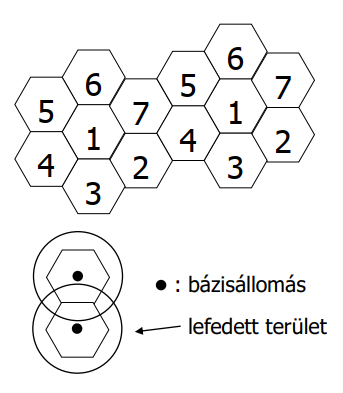
\includegraphics[width=0.28\textwidth]{src/Cella}
\end{center}
\begin{itemize}
	\item Kissebb cellák:
	\begin{itemize}
		\item \textbf{előnyei:}
		\item kis adóteljesítmény elég
		\item nagyobb forgalom bonyolítható adott területen
		\item \textbf{hátrányai:}
		\item sok bázisállomás kell
		\item költséges
	\end{itemize}
\end{itemize}
\subsection{1G rendszerek:} 1970, Analóg rendszer, nem kompatibilis hálózatok, Kb 450MHz, nagy (30-50km) cellák.\\Skandinávia 1981, Hazánkban 1990-2003
 \subsection{2G (GSM):} 1990, Digitális rendszer, legelterjettebb a GSM\\Vannak/voltak más 2G rendszerek is (pl.: USA DAMPS: Digital AMPS)
 \newpage
\section{GSM}
\begin{itemize}
\item GSM: eredetileg: „\textbf{G}roupe \textbf{S}péciale \textbf{M}obile”, később: „\textbf{G}lobal \textbf{S}ystem for \textbf{M}obile communications" \\ \\
európai szabvány (!): az ETSI készítette
új koncepciók a GSM-ben:
\begin{enumerate}
	\item közös, egységes rendszer Európában
	\item hívó fél fizet csak
	\item roaming
	\item SIM kártya (előfizető adatai készülékfüggetlenek)
	\item SMS
	\item titkosított beszédátvitel
\end{enumerate}
\item Digitális átvitel: beszédkódoló (A/D átalakító) a telefonkészülékben, adatátvitel, beszédátvitel egyaránt lehetséges
\item  Sugárzási teljesítmény: max 2 W, adaptív: a minimális
szükségessel ad a végberendezés
\item Cella átmérője: 0,5 – 35 km, tervezői döntés az adott tartományon belül, függ a frekvenciától, forgalomsűrűségtől, terjedési viszonyoktól
\subsection{GSM 900 (Primary-GSM, P-GSM)}
\begin{itemize}
	\item Mobil adó kb 900MHz, bázisállomás is kb 900Mhz
	\item e tartományban kisebb frekvencia kisebb csillapítást szenved,
	így kisebb teljesítményt igényel, ezért a mobil adóé az alsó sáv
	\item 25 MHz-es sáv, egy vivő 200 kHz: 124 vivő (FDMA), ezen a helyi szolgáltatók osztoznak
	\item vivőnként 8 db időrés (TDMA)
	\item 40*8/10 $\approx$ 32 csatorna / cella $\rightarrow$ kb 32 egyidejű beszélgetés $\rightarrow$ elég kevés
	\item Beérkező hívás esetén egy közös jelzéscsatornán értesíti erről a
	végberendezést
	\item Kimenő hívás esetén egy másik közös jelzéscsatornán kezdeményez a
	mobil
	\item \textbf{országos lefedésre alkalmas a technológia}
\end{itemize}
\subsection{GSM 1800}
\begin{itemize}
	\item Mobil adó kb 1800MHz, bázisállomás is kb 1800Mhz
	\item 75 MHz-es sáv (plusz háromszoros kapacitás!)
	\item de: rosszabb a hullámterjedése (egyenes terjedés, gyorsabb csillapodás)
	\item \textbf{emiatt országos lefedésre nem, csak nagy forgalmú kis területek
	ellátására alkalmas}
\end{itemize}
\item Kétnormás készülékek automatikusan váltanak frekvenciatartományt
\item \textbf{GSM átadás} (handover, handoff) mobil végberendezés átmegy egy másik cellába
\begin{itemize}
	\item eközben nem szakad meg a kapcsolat, de ez történhet:
	\item a mobil végberendezés irányításával: méri, mikor erősebb
	egy másik cella jele
	\item a hálózat irányításával: az dönt a jelerősség és esetleg más
	információk (pl. cella terheltsége) alapján
	\item a hálózat irányításával, a mobil készülék segítségével: a
	hálózat megkéri a végberendezést, hogy küldjön jelerősségi
	információt, de a döntést a hálózat hozza – ez van a GSMben
\end{itemize}
\end{itemize}
\begin{center}
	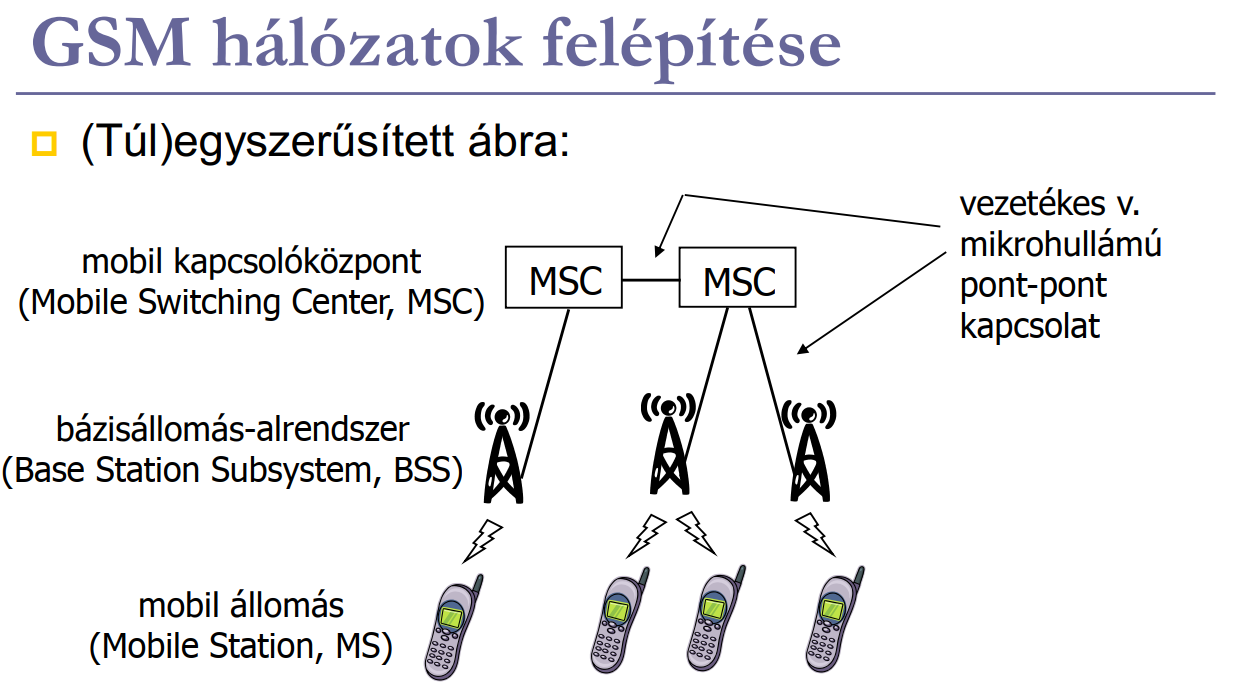
\includegraphics[width=0.9\linewidth]{src/GSMhalozat}
\end{center}
	\section{GSM hálózatok felépítése}
\begin{enumerate}
	\item Bázisállomás-alrendszer
	\begin{itemize}
	\item Bázisállomás (BTS): \\
	egy vagy több elemi adó/vevő \\
	(elementary transmitter/receiver)
	\item ázisállomás-vezérlő (BSC):
	\\egy vagy több bázisállomást vezérel
	\\kapcsolás (beszédcsatornák összekötése)
	\\rádiócsatorna-hozzárendelés
	\\hívásátadás-vezérlés
	\end{itemize}
	\item Hálózati alrendszer
	\begin{itemize}
		\item Mobil kapcsolóközpont (MSC)
		\\egy „hagyományos” telefonközpont
		\\mobil-specifikus bővítésekkel
		\\autentikáció, helyzetnyilvántartás, hívásátadás BSC-k között, barangolás
		\item MSC tartalmazza a látogatói helyregisztert (VLR)
		\\A HLR információinak egy részét tárolja ideiglenesen (ami a hívásfelépítéshez szükséges) az
		ott tartózkodó mobil állomásokról
		\item Honos helyregiszter (HLR)
		\\ előfizetőre vonatkozó adatok, szolgáltatási jogosultságok, aktuális
		tartózkodási hely
		\\ egy HLR hálózatonként
		\item AuC: hitelesítő központ (Authentication Center)
	\end{itemize}
\end{enumerate}

\subsection{Azonosítók a GSM-ben}
\begin{enumerate}
	\item \textbf{MSISDN:} Mobile Station ISDN Number, mobil állomás
	ISDN szám
	\begin{itemize}
		\item a jól ismert mobil telefonszám
		\item egyedi a világon
		\item  MSISDN = országkód (Mo.: 36) + hálózatkijelölő szám
		(Mo:20/30/70) + előfizetői szám
	\end{itemize}
	\item \textbf{IMSI:} International Mobile Subscriber Identity,
	nemzetközi mobil előfizető azonosító
	\begin{itemize}
		\item GSM hálózatokban elsősorban ez azonosítja az előfizetőt: az
		adatbázisok ezzel vannak indexelve
		\item a SIM kártyához van rendelve
		\item egyedi a világon
		\item IMSI = mobil országkód (Mo: 216) + mobil hálózati kód
		(Mo.:01/30/70) + 10 jegyű mobil előfizető azonosító szám
		\item szolgáltatóváltásnál az MSISDN maradhat, de a SIM kártyát és
		ezzel együtt az IMSI-t cserélni kell 
	\end{itemize}
	\item \textbf{MEI:} International Mobile Equipment Identity,
	nemzetközi mobilkészülék-azonosító
	\begin{itemize}
		\item  végberendezést azonosítja
		\item egyedi a világon
		\item IMEI = <készülékazonosító> (8 jegyű) + <gyári szám> (6 jegyű)
		+ <ellenőrző számjegy> (1 jegyű) (+<szoftver verzió>)
		\item Lekérdezése: $*\#06\#$
	\end{itemize}
	\item \textbf{MSRN:} Mobile Station Roaming Number, barangoló szám
	\begin{itemize}
		\item egy VLR-hez tartozó helyi címtartományba tartozó telefonszám,
		amit az arra járó GSM készülék ideiglenesen használ
		\item a felhasználó számára transzparens, nem látszik
		\item ez teszi lehetővé, hogy a szám utaljon a földrajzi helyre: ebből a
		számból már tudni, hogy merre kell keresni az adott készüléket,
		ha felhívja valaki
	\end{itemize}
\end{enumerate}
\subsection{Végberendezés helyének nyilvántartása}
Hogyan? cella szinten? Országis szinten?\\
Kompromisszum: "Location Area"\\
\begin{itemize}
	\item néhány (tipikusan 20-30) cella együttese
	\item köztük való cellaváltáskor nincs helyzetfrissítés (Location update)
	\item Location Area váltáskor helyzetfrissítés
	\item bejövő híváskor/SMS-kor broadcast keresési üzenet (paging) a Location
	Area-ban
	\item Alapból ennél pontosabban nem tárolja a hálózat, hogy hol vagyunk!
\end{itemize}
\begin{center}
	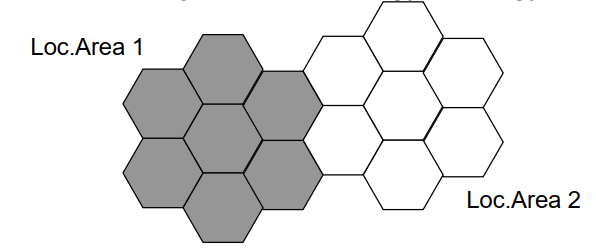
\includegraphics[width=0.5\linewidth]{src/LocArea}
\end{center}
\subsection{GSM szolgáltatások}
\begin{enumerate}
	\item  \textbf{Beszédátvitel: }
	\\kodek sebessége 13 kb/s (később: 5,6 kb/s is)
	\\ kompromisszum: viszonylag gyenge hangminőség, jobb
	frekvenciakihasználtság
	\item \textbf{SMS} (Short Message Service, rövid szöveges üzenet szolgáltatás)
	\\ 160 karakter max.
	\item \textbf{Adatátvitel:} kezdetben 9,6 kb/s, később 14,4 kb/s, majd ez folyamatosan nőtt....
	\item\textbf{MMS} (Multimedia Messaging Service, multimédia üzenetküldő szolg.)
	\\ multimédia üzenet: kép, írott szöveg, hang együtt
	\\ 2002-től elérhető szolgáltatás, néha ma is használják
\end{enumerate}
\section{GSM/GPRS: „2,5 G”}
\begin{itemize}
	\item  GPRS (General Packet Radio Service, általános
	csomag alapú rádiós szolgáltatás)
	\item \textbf{csomagkapcsolt adatátvitel}, a GSM kiegészítése
	\item előny: jobb kihasználtság, fizetés kilobájt alapon, nem perc szerint
	\item adatsebesség kb. 60-80 kb/s
\end{itemize}
\subsection{Áramkörkapcsolás („vonalkapcsolás”, circuit switching)}
\begin{itemize}
	\item klasszikus telefonhálózatokban van ilyen
	\item végponttól végpontig \textbf{garantált minőségű} csatorna
	\item \textbf{hívásfelépítés} a kommunikáció előtt
	\item \textbf{lebontás} a kommunikáció után
	\item a csatornát csak a hívó és a hívott használhatja
	\item ha épp nem beszélnek, üres a csatorna
	\item lehet fizikailag egy áramkör, de lehet általánosabb értelemben
	egy csatorna
\end{itemize}
\subsection{Csomagkapcsolás (packet switching)}
\begin{itemize}
	\item az átvitt információt kis csomagokra bontva továbbítjuk
	\item nem kell hívásfelépítés, bontás
	\item előny: \textbf{statisztikus multiplexelés}
	\\ ha épp nincs kommunikáció, más is használhatja a csatornát
	\\ olcsóbb!
	\item hátrány: minőség nem garantált, (Quality of Service, QoS) biztosítása külön feladat
\end{itemize}
\begin{center}
	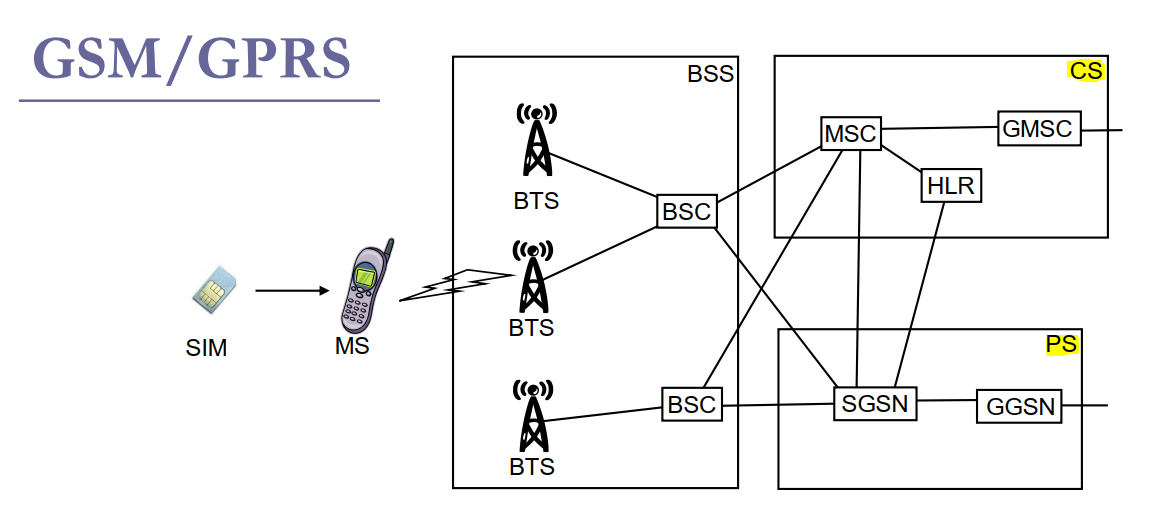
\includegraphics[width=0.5\linewidth]{src/gsmgprs}
\end{center}

\subsection{EDGE: „2,75 G” (Enhanced Data Rate for Global/GSM Evolution)}
\begin{itemize}
	\item javított modulációs eljárás: eredetileg 1 bit/szimbólum $\rightarrow$ EDGE: 8PSK, 3 bit/szimbólum 
	\item háromszoros adatátviteli sebesség\\ez csak jobb jel/zaj viszony esetén működik
	\item adatsebesség kb. 150-180 kb/s
\end{itemize}
\section{Mobiltelefon-hálózatok: UMTS}
Universal Mobile Telecommunications System, Egyetemes mobil távközlési rendszer\\
célok:
\\ GSM-nél jobb beszédhangminőség, frekvenciakihasználtság, nagyobb adatátviteli sebesség, GMS kompatibilitás
\subsection{UMTS szolgáltatások}
\begin{itemize}
	\item Beszédátvitel: Adaptive MultiRate (AMR) kodek, 4,7 – 12,2 kb/s
	\item Adatátvitel, Internet elérés (sima 3G)
	\begin{itemize}
		\item városban tipikus max. 384 kb/s
		\item vidéken tipikus max. 144 kb/s\\
		\small{(GSM: kb. 14 kb/s, GSM/GPRS: kb. 50-80 kb/s, EDGE+GSM/GPRS: kb. 150-180 kb/s)}
	\end{itemize}
\item Multimédia szolgáltatások (IP nélkül 3G felett)
\begin{itemize}
	\item videotelefonálás – nem sokan használják
	\item TV adások közvetítése, rádióhallgatás, filmek, zenék letöltése –
	nem váltak be
\end{itemize}
\end{itemize}
\begin{center}
	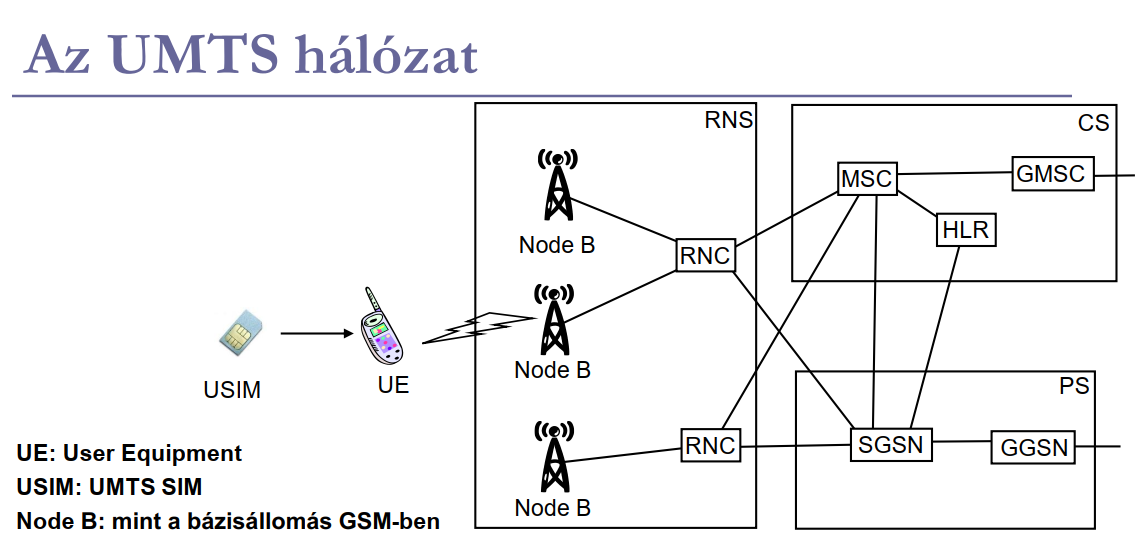
\includegraphics[width=0.6\linewidth]{src/umtsnetw}
\end{center}
\subsection{Duplexitás kezelés}
fel- és lefele irányú adatok elkülönítése\\
Alkalmazott lehetséges megoldások: \textbf{időben, rekvenciában}
\begin{itemize}
	\item  Mindkettőt használják UMTS-ben (de nem egyszerre) 1885-2025 és 2110-2200 MHz:
	\item FDD: Frequency Division Duplexing
	\begin{itemize}
	\item nagyobb frekvencia a lefele irányban (nagyobb csillapítás $\rightarrow$
	nagyobb teljesítmény kell)
	\end{itemize}
	\item  TDD: Time Division Duplexing
	\begin{itemize}
	\item a fel- és letöltés időben váltakozik ugyanabban a frekvenciasávban
	\item előnye: a fel/letöltés aránya dinamikusan változtatható az aktuális
	igények függvényében
	\end{itemize}
\item Nagy frekvencia: csupán pár (3-5) km átmérőjű cellák
\item  A frekvenciákat 5 MHz-es csatornákra osztják, melyekben \textbf{CDMA}-t
használnak
\item \textbf{CDMA}, Code Division Multiple Access, kódosztásos többszörös
hozzáférés (KH1 tárgy már érintette) (SD-CDMA)
\item Ugyanaz a frekvencia, ugyanaz az idő, más kód
\item Minden jel „szétkenve” a teljes spektrumra, de kis teljesítménnyel
\end{itemize}
\begin{center}
	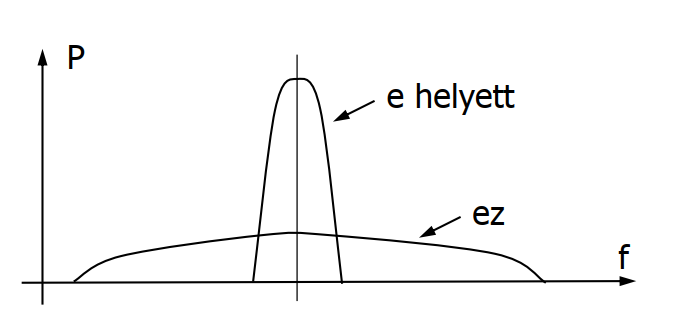
\includegraphics[width=0.7\linewidth]{src/CDMA}
\end{center}
\subsection{UMTS kódosztás}
A kódolás két menetben történik
\begin{itemize}
	\item nulladik lépés a csatornakódolás (channel coding) ez nem ugyanaz, mint a csatornázási kódolás, ez hibajavító kódolás (avagy előremenő hibajavítás, forward
	error correction, FEC)
	\item csatornázási kód (channelisation code) kiterjesztés / spreading néven is fut
	\item keverő kódolás (scrambling)
	\item utána jön a rádiófrekvenciás modulálás, kisugárzás
\end{itemize}
\subsubsection{Csatornázási kód}
\begin{itemize}
	\item Működés: DS-CDMA (Direct Sequence CDMA, közvetlen sorozatú
	CDMA)
	\subitem a digitális jelet összeszorozzuk egy ún. szóró kóddal (spreading
	code), és ezt sugározzuk ki
	\subitem a szorzás pontosabban: NOT(XOR(bit1,bit2))
	\subitem a kisugárzott jel hozzáadódik a többi adó által kisugárzotthoz
	\item A szóró kód bitsebességge (chiprate) sokkal nagyobb (kb. 100x)
	\item A szóró kódok ortogonálisak, azaz egy bitidőre átlagolva két
	szórókód szorzatát nullát kapunk
\end{itemize}

	\subsubsection{Kódosztás}
	\begin{itemize}
	\item  STEP 1. A szóró kódot és az elkódolni kívánt adatot is reprezentáljuk a
	következőképp:
	\subitem  1 $\rightarrow$ 1
	\subitem  0 $\rightarrow$ -1
	\subitem  Vegyük észre: ekkor NOT(XOR(a,b)) valójában a*b, azaz szorzás
	\subsubitem 1*1=1, 1*-1=-1, -1*1=-1, -1*-1=1
	\item  STEP 2. Végezzük el a szóró kód összeszorzását a küldendő adattal
	\subitem  a szóró kód összes bitjét szorozzuk az adat egy adott bitjével, így jelentősen megnő
	a jelsebesség
	\item  STEP 3. Sugározzuk ki az így kapott jelet a közös frekvencián
	\subitem  Modellünkben egyszerűen összeadjuk az összes így kapott jelet
	\subitem  Dekódolás
	\item  STEP 1. A vett jelet (a kódolás STEP 3 összege) szorozzuk meg az adó szóró
	kódjának a bitjeivel sorban. Ahány bitet kívánunk venni, annyiszor ismételjük
	ezt meg
	\item  STEP 2. Az így kapott értékeket átlagoljuk bitidőkre
	\item  STEP 3. Ha az átlag 1: a küldött bit 1. Ha az átlag -1: a küldött bit 0
	\item  STEP 4. Ismételjük meg mindezt az összes vevőre
\end{itemize}
Kódosztásos példa, számolás 3Gs jegyzetben 15.o
-- 
\subsubsection{OVSF (Orthogonal Variable Spreading Factor)}
\begin{itemize}
	\item Tökéletesen ortogonális kódszavak
	\item  Nevük: Ortogonális, változtatható kiterjesztési faktorú (Orthogonal
	Variable Spreading Factor,OVSF) kódok, avagy \textbf{Walsh kódok}
	\subitem  Azonban az ortogonalitás csak akkor teljesül, ha pontosan egy
	fázisban vannak a kódok
	\item nem azonos kezdőfázis esetén sem magával, sem másik kóddal nem
	nulla a korrelációja
	\item azaz közös órajel kell
	\subitem  Gyakorlatban: azonos adó különböző csatornáinak elválasztására
	használják
	\item Node B-ben: különböző végberendezéseknek szóló jelek elkülönítésére
	\item Végberendezésben: jelzés és adatjelek elkülönítésére
	\begin{center}
		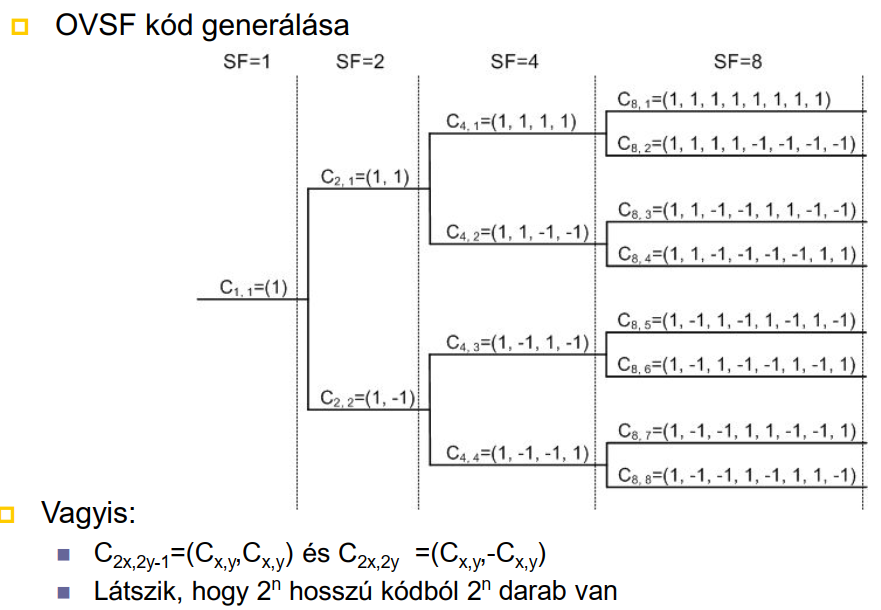
\includegraphics[width=0.55\linewidth]{src/OVSF}
	\end{center}
\item E kód a keskenysávú bemenő jelet szélessávúvá alakítja
\subitem A kiterjesztési faktor változik 4 és 512 között
\item azt adja meg, hogy hányszorosa lesz a chipsebesség a
bitsebességnek
\item másképpen: hány chip hosszú egy szóró kód
\item ismét másképp: hány db. szóró kód van
\subitem A chipsebesség viszont mindig fix: 3 840 000 chip/sec
\item azaz 3,84 MChip/s, 3,84 Mcps
\subitem Tehát kisebb adatsebességhez nagyobb kiterjesztési
faktor tartozik, nagyobb adatsebességhez kisebb
\item több hosszabb kód van, kevesebb rövidebb
\item azaz kisebb adatsebességből többet tudunk küldeni egyszerre,
nagyobb sebességből kevesebbet, a szorzat állandó
\end{itemize}
\subsubsection{Keverő kódolás}
\begin{itemize}
	\item Csak kvázi ortogonálisak egymásra, ugyanakkor önmaguk időbeli
	eltoltjára is kvázi ortogonálisak
	\subitem Fajtájuk ún. pseudo-noise, „ál-zaj” kódok, nevük \textbf{Gold kód}
	\subitem Célja az adóberendezések megkülönböztetése. Adónként van egy
	ilyen kód
	\subitem lefele irány: cellák (azaz Node B-k) elkülönítése
	\subitem felfele irány: végberendezések elkülönítése
	\subitem Nem igényelnek szinkronizációt a források között
	\subitem „Cserébe” nem teljes az ortogonalitás: a vevő az egyik forrás jelének
	dekódolásakor a többi forrás jelét enyhe zajnak érzékeli
	\subitem A cella kapacitását itt az szabja meg, hogy meddig nem zavaró még
	ez a zaj a dekódolásban
	\subitem Ez nem egy fix korlát!
	\subitem A GSM FDMA/TDMA rendszerében a vivők/időrések száma fix korlátot
	adott
\end{itemize}
\subsubsection{Összefoglalás}
\begin{tabular}{|c|c|c|}
	\hline 
	& csatornázási kód & keverőkód \\ 
	\hline 
	cél & forráson belüli adatfolyam elkülönítése & források elkülönítése \\ 
	\hline 
	kódhossz & 4..256 chip fel, 4..512 chip le & 38400 vagy 256 chip fel, 38400 chip le \\ 
	\hline 
	kiterjesztés & van, növeli az adási sávszélességet & nincs \\ 
	\hline 
	ortogonalitás & tükéletes & nem tökéletes \\ 
	\hline 
	szinkronizáció & szükséges & nem szükséges \\ 
	\hline 
\end{tabular} 
\subsection{UMTS teljesítményszabályozás}
\begin{itemize}
	\item Nem tökéletes az alkalmazott keverő kód ortogonalitása
	\item Emiatt más egy adott mobil eszköz jelét figyelve a bázisállomáson a
	többi mobil jele zajként jelentkezik
	\item Ezért az kell, hogy minden mobil jele kb. egyforma teljesítménnyel
	érkezzen a Node B-hez
	\subitem különben az erősebb jel elnyomja az összes gyengébbet
	\item Megoldás: Node B felszólítja a mobil eszközt a teljesítmény
	növelésére/csökkentésére
	\item 1500/sec gyakorisággal(!)
	\subitem Különben pl. egy épület mögül előbukkanó, eddig erősen adó eszköz
	tönkretenné az egész cella kommunikációját
	\item GSM-ben is van ilyen:
	\subitem telep kímélésére, élettani kockázat csökkentésére
	\subitem más, távoli de azonos frekin üzemelő cellákkal való interferencia
	elkerülésére
	\subitem 2/sec gyakorisággal (!)
\end{itemize}
\subsubsection{UMTS cellalélegzés}
Több felhasználó egy cellában
\begin{itemize}
\item $\rightarrow$ nagyobb „háttérzaj”
\subitem hisz nem tökéletesen ortogonálisak a keverő kódok
\item $\rightarrow$ kisebb cella használható csak effektíven
\subitem a távol lévő állomások kirekesztődnek
\item $\Rightarrow$ a cella mérete változik a forgalomtól függően
\subitem a cella „lélegzik”
\item megnehezíti a cellatervezést
\end{itemize}
\section{HSPA (High-Speed Packet Access, nagy sebességű csomagkapcsolt hozzáférés)}
\begin{itemize}
	\item UMTS továbbfejlesztése nagyobb adatsebességek felé
	\item 2 protokoll közös neve:
	\subitem HSDPA (High Speed Downlink Packet Access, nagy sebességű
	csomagkapcsolt letöltési hozzáférés)
	\item akár 14 Mb/s
	\subitem HSUPA (High Speed Uplink Packet Access, nagy sebességű
	csomagkapcsolt feltöltési hozzáférés)
	\item akár 5,76 Mb/s
	\item Az UMTS része, annak részben továbbfejlesztése
	\subitem 3,5G néven is emlegetik
	\subitem 2010-es évek első éveiben vezették be
	\item A következő lépés: HSPA+
	\subitem elvi max 42 Mb/s le, 22 Mb/s fel
	\subitem „3,75 G
\end{itemize}
\section{4G/LTE: Long Term Evolution}
\begin{itemize}
	\item Negyedik generációs mobilhálózat
	\item \textbf{IP alapú, csomagkapcsolt átvitel}
	\item Nagy sebességű internet biztosítása
	\item Csak internet, hangátvitelhez \textbf{VoLTE} kell (később)
	\item 3 fő szabvány: LTE, LTE-Advanced, LTE Advanced Pro
	\item  Felhasználói igény: Gyorsabb mobil internet, Multimédiás tartalmak, videó letöltése
	\item Operátorok igénye: Új szolgáltatások, jobb szolgáltatásminőség, több előfizető
	kiszolgálása, Gazdaságosabb hálózat üzemeltetés
	\item  Gyártók igénye: új eszközök és szolgáltatások eladása
\end{itemize}
\subsubsection{LTE világszerte}
\textbf{GSM} vs. \textbf{CDMA} szabványú hálózatok
\begin{itemize}
\item CDMA mint... közeghozzáférés vs. szabvány gyűjtőnév
\item Szabványok
\subitem GSM (3GPP): Európai eredetű, ETSI által megalkotva
\subitem CDMA (3GPP 2): Amerikai eredetű, Qualcomm (chipgyártó) által
\subsubitem 2G: CDMAOne | 3G: CDMA2000 / EV-DO
\subsubitem A CDMA szabványú hálózatok már 2G-ben is CDMA-t használtak
közeghozzáférésre ellentétben a GSM-el
\item A mobilkészülékek nem kompatibilisek egymással
\subitem GSM: SIM alapú felhasználó azonosítás
\subitem CDMA: hálózat alapú beengedés szabályozás, telefon alapján
\subsubitem ESN: Electronic Serial Number ($\sim$IMEI)
\item LTE: egységes szabvány, SIM alapú
\subitem Verizon: 2019 végén leállítja 2G/3G CDMA szolgáltatását
\item \textbf{Különböző frekvenciák vannak és nem minden készülék támogat minden frekvenciát}
\end{itemize}
\subsubsection{LTE követelmények}
\begin{itemize}
\item 3G továbbfejlesztések \textbf{(MIMO)}
\subitem \textbf{Csomagkapcsolt hálózatra való optimalizálás}
\subitem IMT Advanced Standards – LTE követelmények
\item\textbf{ „All-IP” csomagkapcsolt hálózat}
\item 100 Mbps gyorsan mozgó / 1 Gbps nem mozgó felhasználónak
\item 5-20 MHz skálázható sávszélesség
\item \textbf{Együttműködés korábbi (2G/3G) rendszerekkel}
\subitem Ezen követelményeket majd az LTE Advanced teljesíti
\item Erre hivatkozunk, mint az igazi „4G” rendszer
\end{itemize}
\subsection{Tulajdonságok}
\begin{itemize}
	\item Rádiós késleltetés max 5 ms
	\item 1-5 km sugarú cellák
\end{itemize}
\subsubsection{OFDMA: Orthogonal Frequency Division Multiple Access}
	\begin{itemize} 
		\item Változó sélességű spektrumallokáció: 1.4, 3, 5, 10, 15 vagy 20 MHz vivő
		\item Alvivők (15 kHz) átlapolódhatnak
	\end{itemize}
\subsubsection{MIMO (Multiple In, Multiple Out)}
	\begin{itemize}
		\item MIMO: adatsebesség növelése az
		adatküldés párhuzamosításával
		\item  Több antenna a bázisállomásban és
		a készülékekben is
		\item  Ugyanaz a frekvencia és idő, de
		más adatfolyam megy át
		\item  Massive MIMO: 8-nál több antenna
		\item  \textbf{MU-MIMO (Multi User MIMO):} egyszerre nem csak egy klienst szolgál ki időben osztott módon
		\item \textbf{Beamforming:} mobil / WiFi kliens
		tudatja a helyét a bázisállomással /
		routerrel, aki irányítottan sugároz
		felé vezérelve a jel fázisát és
		amplitudóját/jelszintjét
		\subitem  Jobb sávszélesség kihasználás,
		nagyobb hatótávolság
			\subitem Példa: lámpa búra nélkül vs. búrával
	\end{itemize}
\subsubsection{Cellák}
Többféle cellaméret, interferencia lehetősége
	\begin{itemize}
		\item Heterogén hálózatok (HetNet) / Small Cells
		\item \textbf{Több különböző cellatípus kombinálása, cella a cellában} $\rightarrow$ \textbf{interferencia}
	\end{itemize}
\subsection{LTE technikák}
\begin{enumerate}
	\item Nagyobb adatsebesség
		\begin{itemize}
		\item  OFDMA, alvivők, változó szélességű spektrumallokáció
		\item  64-QAM moduláció
		\item  MIMO \& Beamforming -- küldés párhuzamosítása \& irányított sugárzás
		\item  Vivő aggregáció
		\subitem Több vivő összefogása $\rightarrow$ jobb adatsebesség, kisebb késleltetés
		\end{itemize}
	\item Több felhasználó kiszolgálása
	\subitem  MU-MIMO
	\item Lefedettség \& helyi adatsebesség
		\begin{itemize}
		\item  Small cells – többféle cellaméret, „cella a cellában”
		\item  Relay eNodeB – átjátszó, jelkorrekciós funkció
		\subitem Kis energiafogyasztású „Small cell” a cellahatárnál
		\subitem Donor eNodeB-hez (DeNodeB) kapcsolódik (olyan eNodeB, mely Relay eNodeB-t támogat)
		\end{itemize}
	\item 	Offload (tehermentesítés) \& nagyobb adatsebesség
		\begin{itemize}
		\item  VoWiFi (később)
		\subitem DE! készülék támogatás is kell több technológiához (pl. MIMO, vivő aggr.)
		\end{itemize}
\end{enumerate}
\subsection{LTE architechtúra}
\begin{center}
	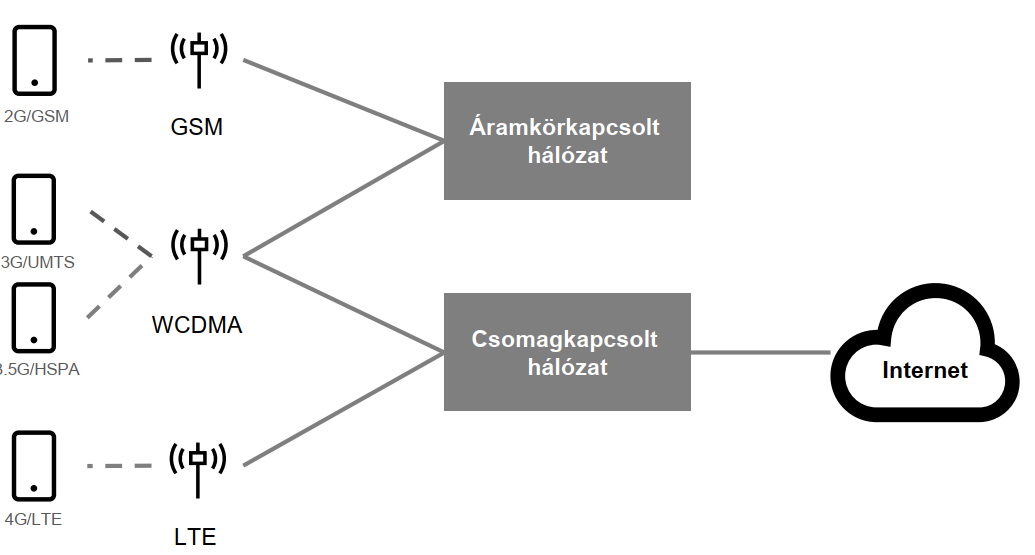
\includegraphics[width=0.5\linewidth]{src/LTEarch}
\end{center}
\begin{center}
	\includegraphics[width=0.8\linewidth]{src/LTEarch2}
\end{center}
\begin{itemize}
	\item \textbf{eNodeB} – LTE bázisállomás
	\subitem Nincs külön Controller
	(pl. RNC 3G-nél)
	\subitem eNodeB része $\rightarrow$ kisebb
	késleltetés
	\item \textbf{SGW} (Serving Gateway)
	\subitem IP adattovábbítás a felhasználó
	és a külső hálózat között
	\subitem Mobilitásban is szerepe van
	\item  \textbf{PGW} = PDN GW (Packet Data
	Network Gateway)
	\subitem Kilépési pont külső hálózatok
	felé
	\subitem IP cím allokáció
	\subitem Házirend/szabályok
	alkalmazása
	\subitem „Charging” támogatása
	\item \textbf{MME} (Mobility
	Management Entity)
	\subitem Felhasználó követés és
	paging (UE felébresztése
	„idle” módból)
	\subitem Csak vezérlő üzeneteket
	kezel, központi vezérlő
	funkció az LTE-ben
	\subitem Mobilitás kezelés
	\subitem Hordozó (bearer) aktiválás
	\subitem SGW választás
	\subitem Authentikáció kezelése
	(HSS)
	\item  \textbf{HSS} (Home Subscriber
	Server)
	\subitem Felhasználói adatok
\end{itemize}
\subsubsection{Vezérlés és felhasználói adat}
\begin{center}
	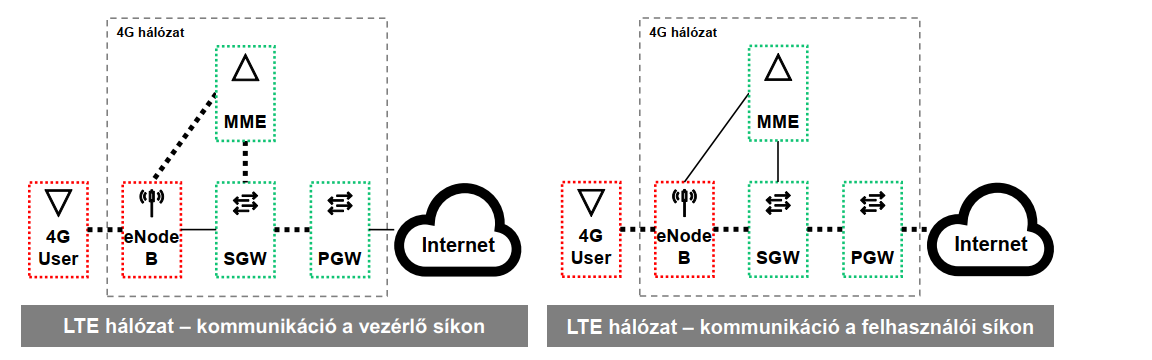
\includegraphics[width=1\linewidth]{src/LTEfelhvvez}
\end{center}
\subsection{LTE handoverek}
Hard handover, mivel…
\begin{enumerate}
	\item Nehézkes a vivő szinkronizáció az OFDMA miatt (resync handovernél)
	\item Controller node hiánya
\end{enumerate}
Mobil készülék mérései alapján az
eNodeB dönt
\textbf{\\Handover típusok:}
\begin{itemize}
	\item Intra-eNodeB Handover
	\subitem Cellaváltás eNodeB-n belül
	\subitem Frekvencia váltás
	\item Inter-eNodeB X2 Handover
	\subitem Közvetlen interfész (X2) szükséges az
	eNodeB-k között
	\subitem MME nem változik, SGW változhat
	\item S1 Handover
	\subitem Ha nincs közvetlen X2 interfész
	\subitem MME és SGW változhatnak
	Bevezető 4G / LTE VoLTE VoWiFi 5
\end{itemize}

\section{VoLTE (Voice over LTE)}
\begin{itemize}
	\item \textbf{Operátorok igénye:}
\begin{itemize}
	\item \textbf{Hang átvitele LTE fölött $\rightarrow$ Voice over LTE (VoLTE)}
\subitem Hanghívás jelenti még mindig a bevételek nagy hányadát
\item Célok:
\subitem Jobbminőségű hangátvitel
\subsubitem HD Voice, kis késleltetés
\subitem Energiahatékonyság
\subitem Gazdaságosabb hálózatüzemeltetés
\subsubitem Új operátoroknál felmerülhet a kizárólag LTE alapú megoldás
\end{itemize}
\item \textbf{VoIP vs VoLTE:}
\begin{itemize}
	\item VoLTE = VoIP?
\textbf{	\subitem IP alapú hangátvitel, garantált minőségű!}
\item VoLTE = LTE + IMS?
\subitem IMS = IP Multimedia Subsystem
\subsubitem Alkalmazás / kapcsolat kezelő / média szerverek (hálózati funkciók)
összessége
\subitem IMS – az egyetlen standard multimédiás szolgáltatás LTE-re
\end{itemize}
\end{itemize}
\subsection{Használati feltételei}
\begin{enumerate}
	\item Hálózati támogatás
	\subitem Speciális chipset
	\item A 2 kapcsolat fenntartása (internet + IMS)
	\item Média kodek támogatás
	\subitem VoLTE feature elérhetősége
	\item SW upgrade
	(példa: Samsung Galaxy S5 – 2014 június)
	\item OS: Android 5+, iOS 8+
	\subitem Telefon beállítások
\end{enumerate}
\subsection{VoLTE architechtúra}
\begin{center}
	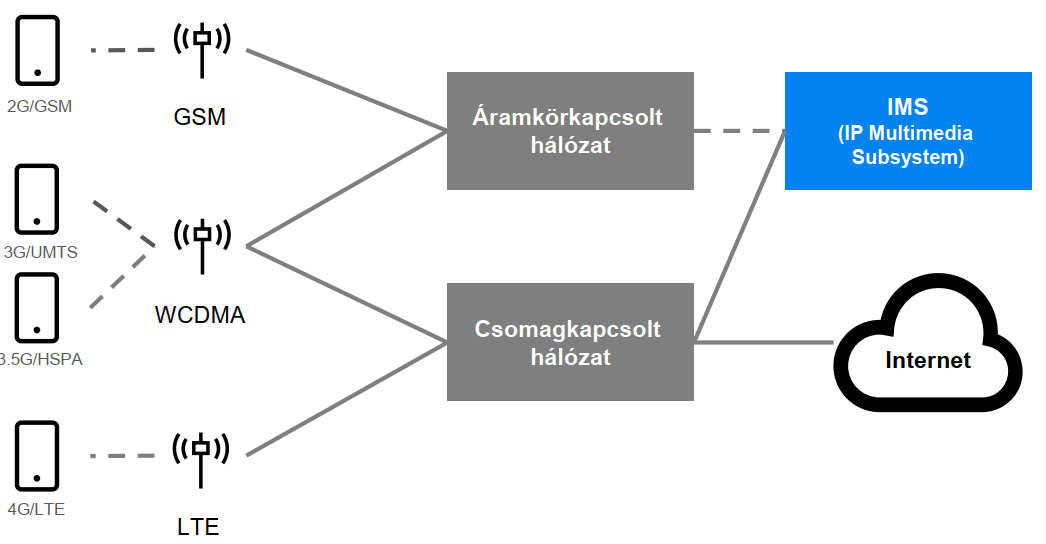
\includegraphics[width=0.7\linewidth]{src/VoLTEarch}
\end{center}
\begin{center}
	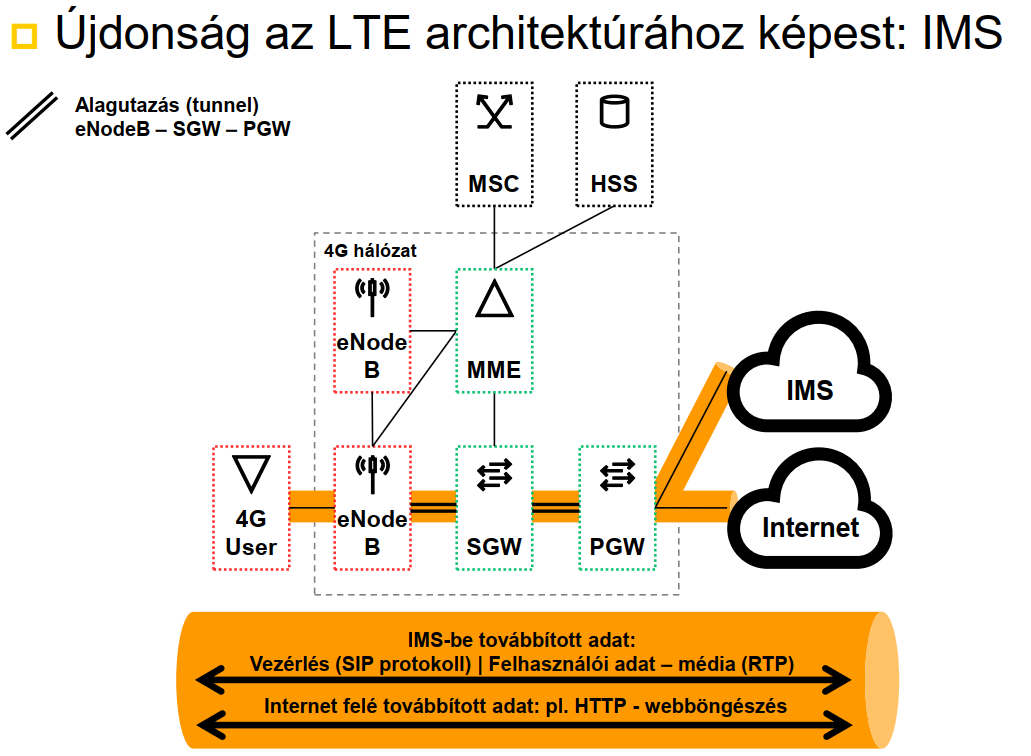
\includegraphics[width=0.8\linewidth]{src/VoLTEarch2}
\end{center}
\subsubsection{LTE hordozók}
\begin{itemize}
	\item LTE emlékeztető: hogyan jut el egy csomag a
	felhasználótól a külső (internet) hálózatba
	\subitem \textbf{Rádiós interfész + alagutak (tunnel-ek) $\rightarrow$ együtt hordozó
	\item \textbf{Hordozó (bearer)}}
	\begin{itemize}
		\item Logikai egység a felhasználói készülék (UE) és PGW között
		\item  Adott végponthoz / szolgáltatáshoz (pl. internet) kapcsolódik
			\subitem APN: Access Point Name – végpont neve
	\end{itemize}
		\item VoLTE
	\begin{itemize}
		\item \textbf{IMS} kezeli a multimédia szolgáltatásokat
	\begin{itemize}
		\item \textbf{SIP vezérlő protokoll + RTP médiacsomagok}
		\item Ezeket az üzeneteket is el kell juttatni az \textbf{LTE gerinchálózaton keresztül az IMS-be} $\rightarrow$ hogyan lehetséges?
			\subitem  Hasonlóan, mint az internet végpont esetében
			\subitem DE! egy hívásnak más\textbf{ QoS (Quality of Service) követelményei} vannak
			\subitem 9 QoS osztály adott csomagvesztési rátával és késleltetéssel
			\subitem QCI = QoS Class Identifier (QoS osztály azonosító)
		\end{itemize}
	\end{itemize}
\item Két hordozó típus:
\begin{enumerate}
	\item\textbf{ Default (alap) – QoS nem garantált}
	\begin{itemize}
		\item Hálózatra csatlakozáskor épül fel
	(úgynevezett \textbf{Attach} procedúra során)
	\item Megmarad a hozzárendelés a hálózat lebontásáig \textbf{(Detach)}
	\item  Több is létrehozható különböző szolgáltatásokhoz, példák:
	\subitem \textbf{LTE:} csak Internet APN-hez tartozó Default hordozó
	 \subitem \textbf{VoLTE:} IMS és Internet APN-hez tartozó két külön Default hordozó
	\end{itemize}
	\item  \textbf{Dedicated (dedikált) – garantált QoS}
	\begin{itemize}
		\item  \textbf{Ideiglenesen épül fel} például audio vagy video híváshoz
	\subitem Hívás végén lebontásra kerül
	\item Mindig valamely \textbf{default hordozóhoz kötődik}
	\subitem Pl. VoLTE hanghíváshoz tartozó dedikált hordozó az IMS APN-hez
	\end{itemize}
\end{enumerate}
\item \textbf{UE} és \textbf{PGW} kényszeríti ki a QoS-t
\subitem Prioritizálás, sávszélesség/forgalomszabályozás
\subitem Forrás/cél IP és port valamint protokoll alapján
Bevezető 4G / LTE VoLTE VoWiFi 5G
	\end{itemize}
\subsubsection{kapcsolódás a hálózathoz}
\begin{center}
	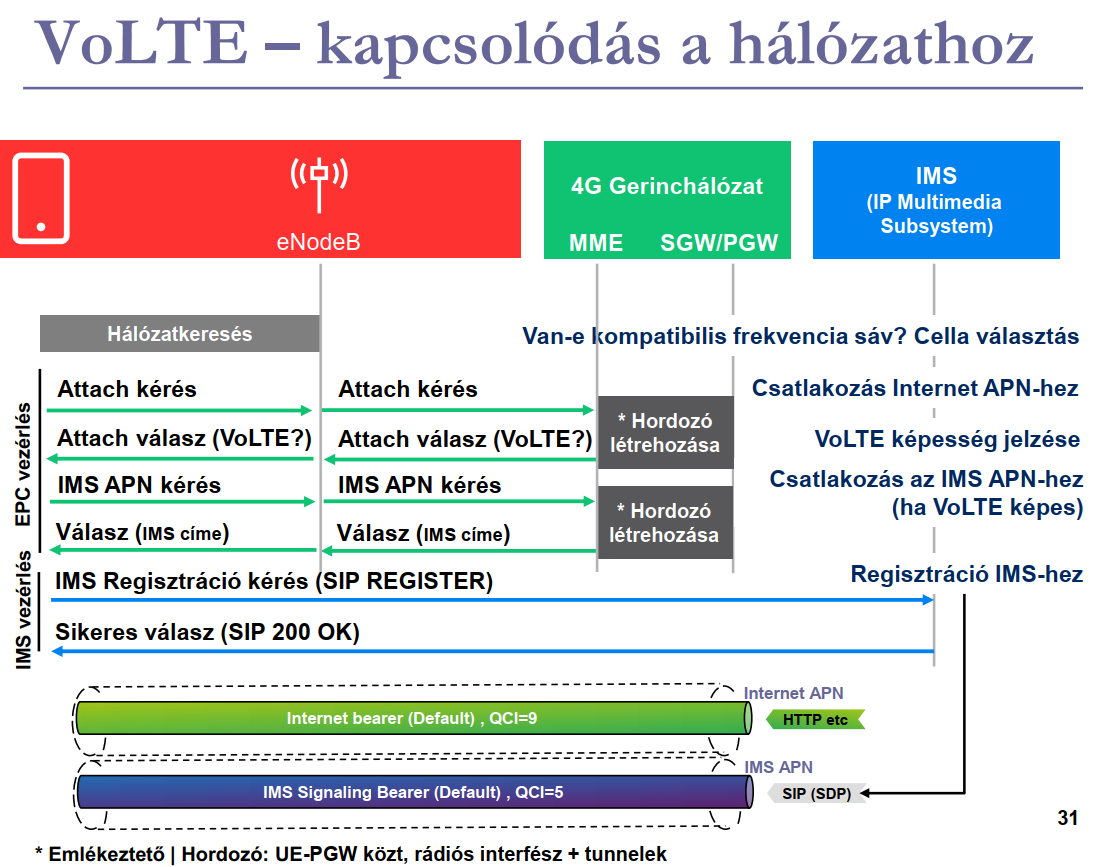
\includegraphics[width=0.65\linewidth]{src/VoLTEkapcsolodas}
\end{center}
\begin{center}
	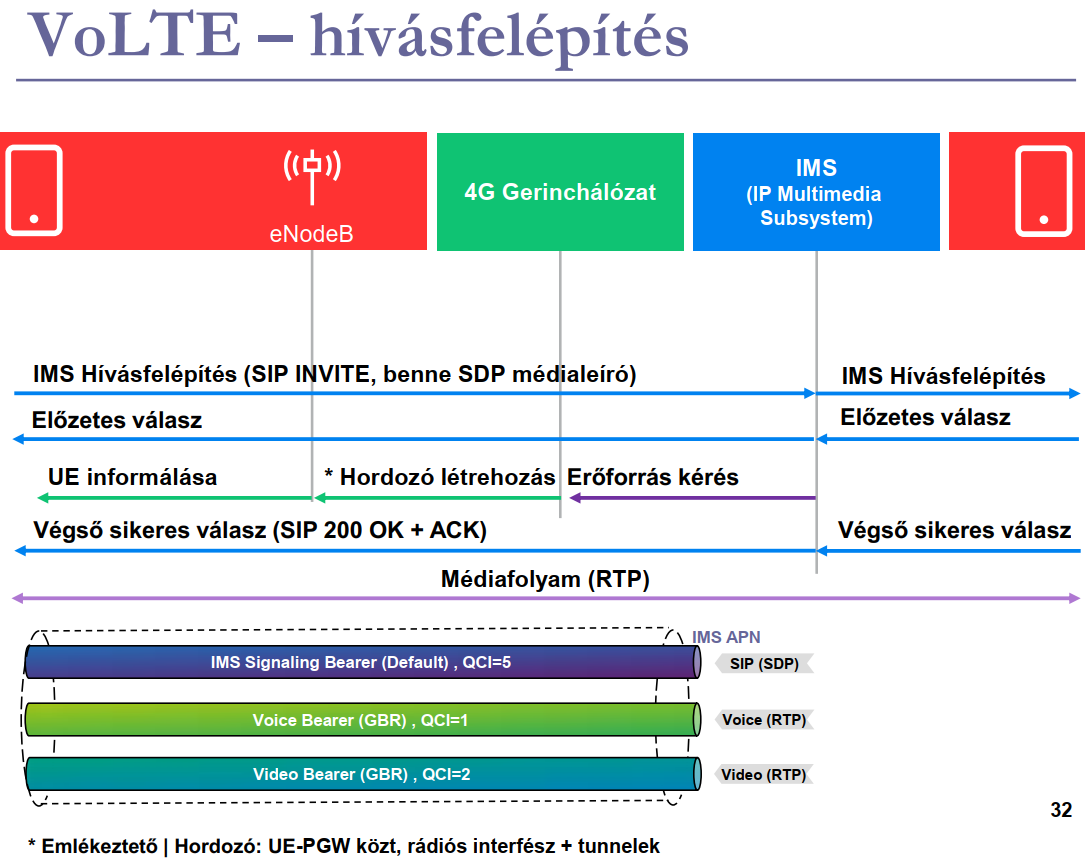
\includegraphics[width=0.65\linewidth]{src/VoLTEkapcsolodas2}
\end{center}
\subsection{VoLTE + 2G/3G?}
\begin{itemize}
	\item \textbf{ICS (IMS Centralized Services)}
		\subitem Multimédia szolgáltatás az IMS-től 2G/3G-n is
\item \textbf{CSFB (Circuit Switched Fall Back)}
\begin{itemize}
	\item Hívásindításkor fallback 2G/3G-re
\item Hívásfogadáskor a „paging” (UE felébresztése) LTE-n történik
\item Adatkapcsolat – 2 opció
\subitem  Megszakad amíg a hívás be nem fejeződik
\subitem  2G/3G-re átkerül $\rightarrow$ lassabb adatsebesség
\item Attach szükséges 2G/3G és 4G rendszerhez is
\item Nagy hívásfelépülési idő
\end{itemize}
\begin{itemize}
\item\textbf{ SRVCC (Single Radio Voice Call Continuity)}
\item Hívás közben handover 4G-ről 2G/3G-re a hívás
megszakadása nélkül
\item \textbf{rSRVCC (Reversed SRVCC):} 2G/3G-ről 4G-re
\item \textbf{UE} az \textbf{Attach} során jelzi, hogy támogatja-e az \textbf{SRVCC}-t
\end{itemize}
\end{itemize}
\subsection{VoLTE összefoglaló}
\begin{itemize}
	\item VoLTE = LTE + IMS + specifikus
	követelmények a hálózat különböző részeire
	\item  Hordozók
	 \subitem Internet APN – internetes adatcsomagok továbbítása
	 \subitem IMS APN – multimédiás (pl.hang) szolgáltatások
	\subsubitem  Vezérlés: SIP (a default/alap hordozón)
	\subsubitem Felhasználói adat: RTP (dedikált hordozón)
	\item  Hálózathoz kapcsolódás és hívásfelépítés
	lépései
	\item  2G/3G kompatibilitás
	 ICS, CSFB, SRVCC
\end{itemize}
\section{VoWiFi – Voice over WiFi}
	\begin{itemize}
		\item Motiváció
		\begin{itemize}
			\item Otthoni beltéri lefedettség – VoLTE hívás problémás
		lehet $\rightarrow$ lefedettség kiterjesztés
		\item 4G cellák és frekvenciahasználat csökkentése
		(offload)
		\end{itemize}
		\item  Opciók
		\begin{itemize}
			\item LTE Femtocellák (3G femtocellák cseréje)
		\item VoWiFi
		\subitem  Kiegészítő szolgáltatásként
		\subitem Szolgáltatás folytonosság WiFi kihasználásával
		\subsubitem Meglévő infrastruktúra
		\subsubitem Telefonnak támogatnia kell (pl. iOS 8+)
		\end{itemize}
	
	\item  \textbf{Előnyök}
		\begin{itemize}
		\item  Nem kell külön alkalmazás
		\item  Meglévő hívószám használata
		\item  Hívásindítás
		 \subitem 2G/3G/VoLTE/WiFi transzparens módon
		\item  Hívás közben
		 \subitem Hívás folytonosság – LTE-VoWiFi vagy WiFi-WiFi handover
		\item  Azonos számlázás, mint VoLTE esetben
		 \subitem Hozzáférés független szolgáltatás
		\item  Nincs roaming díj
		\end{itemize}
	\item \textbf{ Trusted / Untrusted}
		\begin{itemize}
		\item  \textbf{Trusted}: ugyanaz az operátor biztosítja a mobil és WiFi
		szolgáltatásokat
		\item  \textbf{Untrusted}: tetszőleges WiFi hozzáférési pont használata
		\end{itemize}
	\end{itemize}
\subsection{VoWiFi – architektúra („untrusted”)}
	\begin{itemize}
	\item \textbf{ePDG}
		\begin{itemize}
		\item  \textbf{Evolved Packet Data GW}
		\item  Biztonságos kapcsolat (IPSec) kiépítése a 4G készülékkel
		\item  SGW-szerű funkció
		\item  PGW választás
		\item  Mobilitás
		\item  Trusted esetben más funkció ePDG helyett
		\end{itemize}
	\item  \textbf{AAA}
		\begin{itemize}
		 \item  \textbf{Authentication, Authorization, Accounting}
		 \item Biztonsági kulcs
		\end{itemize}
	\item  \textbf{HSS}
		\begin{itemize}
		\item  Felhasználói adatok
		\end{itemize}
	\end{itemize}
\begin{center}
	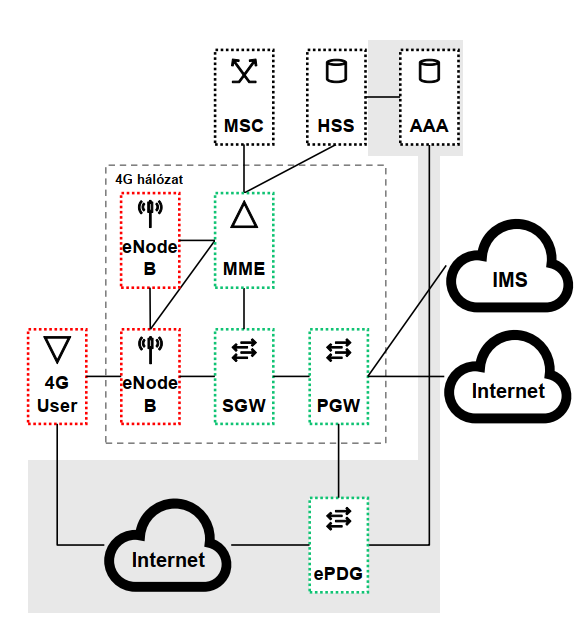
\includegraphics[width=0.42\linewidth]{src/VoWifiarch}
\end{center}
\section{4G $\rightarrow$ 5G (úton az 5G felé...)}
\begin{center}
	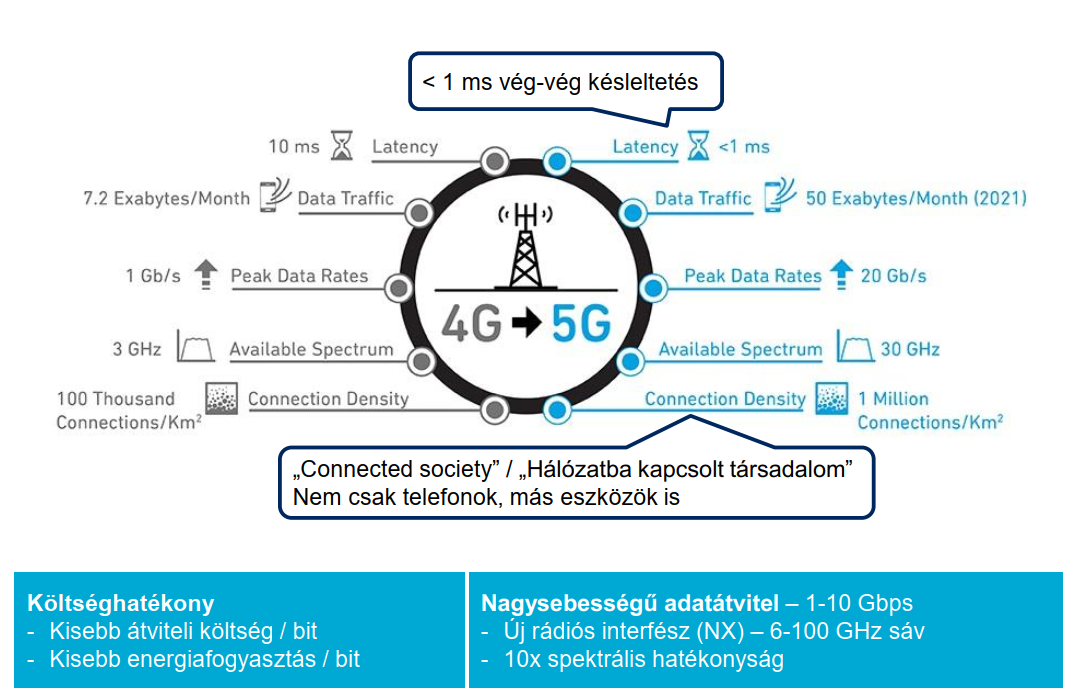
\includegraphics[width=0.7\linewidth]{src/4-5g}
\end{center}
\subsection{5G alkalmazások}
Például:
\begin{enumerate}
	\item Autonomous driving
	\item Augmented reality
	\item Tactile internet
	\item Virtual reality
	\item Critical control of remote devices
	\item \dots
\end{enumerate}
\subsection{CUPS (úton az 5G felé...)}
\begin{center}
	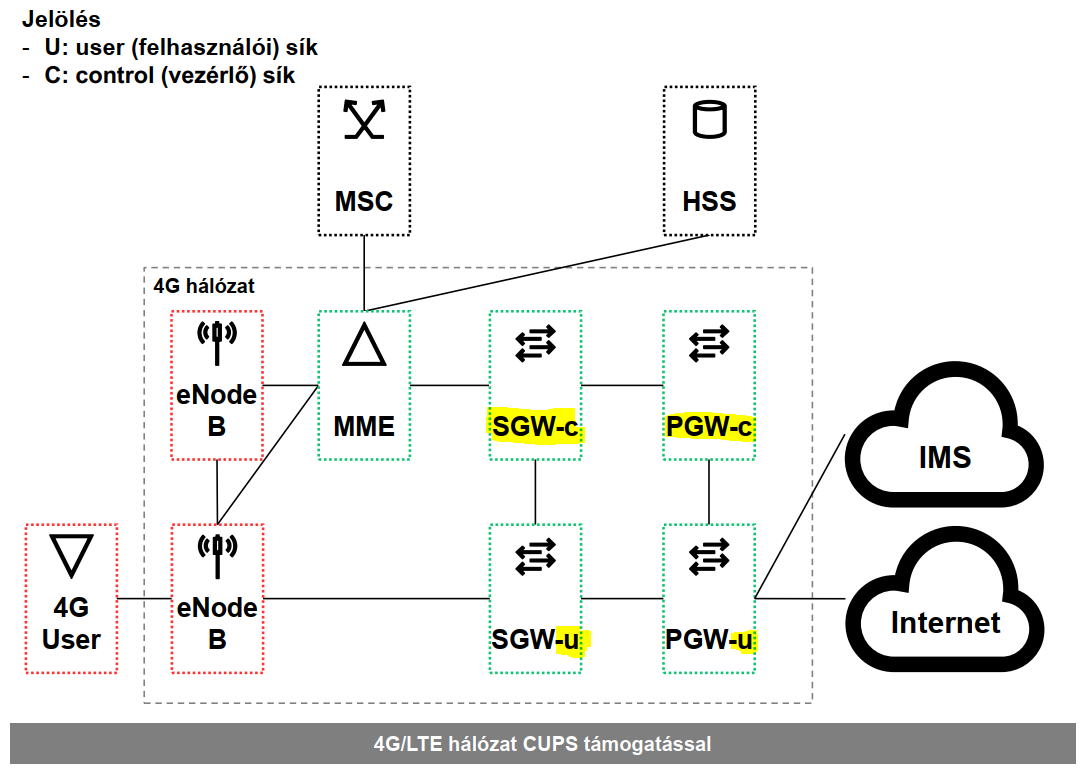
\includegraphics[width=0.6\linewidth]{src/cups}
\end{center}
\begin{itemize}
	\item \textbf{CUPS (Control and User Plane Separation)}
	\subitem  Vezérlő és felhasználói adat \textbf{síkok elkülönítése}
	\subitem  \textbf{Skálázhatóság javítása}
	\item Példák:
	\subitem  \textbf{Vezérlés:} IoT – sok eszköz, eszközönként kevés forgalom
	\subitem  \textbf{Felhasználói adat:} új adatcsomag, pl. ingyen YouTube
\end{itemize}
\begin{itemize}
	\item Access Network / Hozzáférési hálózat
\begin{itemize}
	\item LTE-nél már látott megoldások, azok továbbfejlesztései
	\subitem\textbf{ MIMO, Vivő aggregálás, Beamforming, LTE-U} továbbfejlesztése
	\subitem Rugalmas spektrumallokáció
	\subitem \textbf{Heterogén hálózat / SmallCells}
\end{itemize}
\end{itemize}
\subsection{Core Network / Gerinchálózat}
	\begin{itemize}
		\item Szakítás a telekommunikációs szemlélettel $\rightarrow$ IT
		\item\textbf{ SBA – Service Based Architecture}
			\subitem \textbf{Független szolgáltatások elérése HTTP API-kon kereszül}
		\item \textbf{NFV – Network Function Virtualization}
			\subitem Hálózati \textbf{funkciók virtualizálása}, szoftver – hardware függetlenítés
			\subitem Infrastruktúra megosztása központi adatközpontokban $\rightarrow$ \textbf{költségcsökkentés}
		\item \textbf{SDN – Software Defined Networking}
			\subitem NFV kiegészítése a topológia dinamikus konfigurálásának lehetőségével
		\item \textbf{Network slicing (hálózatszeletelés)}
			\subitem Alkalmazási igények mentén több különböző (pl. Telekom / IoT / Industry)
		gerinchálózat különböző minőségi követelményekkel
	\end{itemize}
\subsection{5G helyzetkép}
	\begin{itemize}
		\item 2016/2017 – 5G teszt
		\begin{itemize}
			\item 800MHz sávszélesség 15 GHz-en (Ericsson \& SK Telekom)
		\subitem 1 Gbps végpontok közötti sebesség
		\subitem 4 ms késleltetés
		\item Handover teszt nagy sebesség mellett (KDDI \& Samsung)
		\item Telekom + Ericsson: első 5G kapcsolat (22 Gbps)
		\end{itemize}
		\subitem Szabványosítás folyamatban
		\begin{itemize}
			\item \item 3GPP: Release 15 (2018) | Release 16 (2019 dec)
		\end{itemize}
		\subitem 2019-ben már kezdeti bevezetés vezető operátoroknál
	\end{itemize}
\begin{center}
	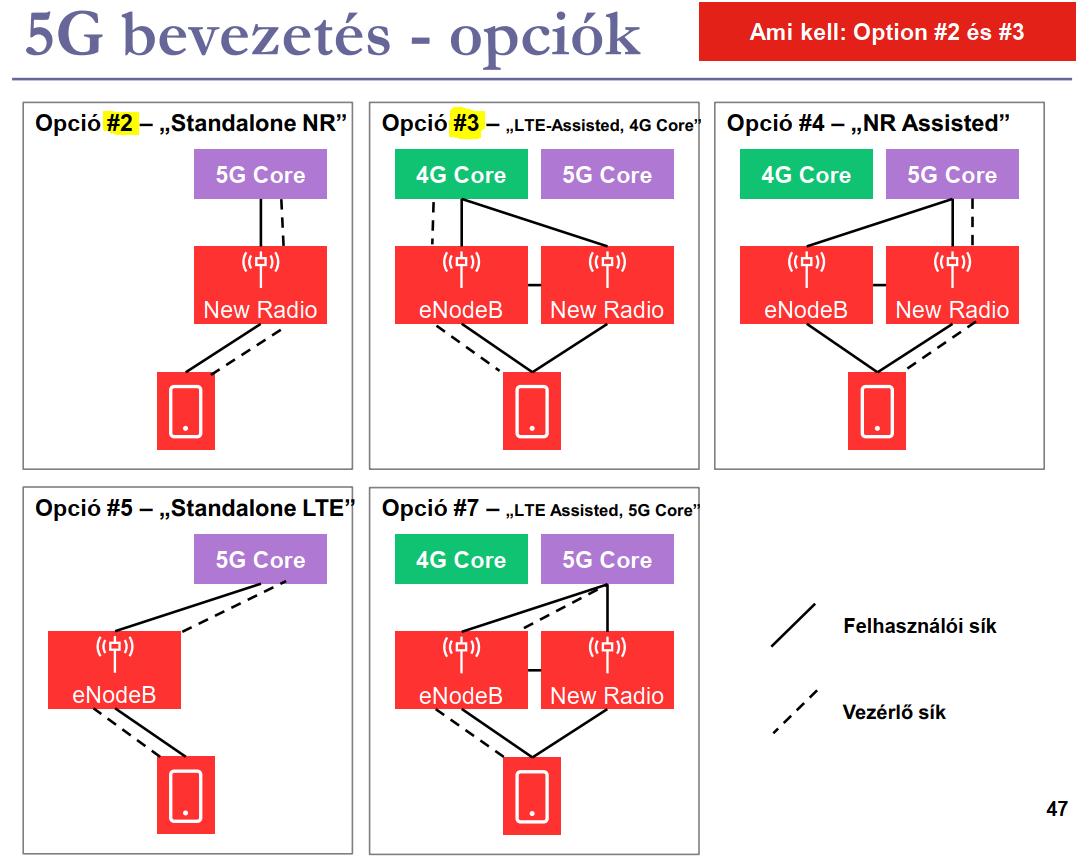
\includegraphics[width=0.6\linewidth]{src/5gopciok}
\end{center}
\section{Rövidítések}
\begin{multicols}{2}
	\begin{minipage}{0.45\textwidth}
	\begin{itemize}
		\item Alapfogalmak
	\begin{itemize}
		\item DL = downlink, letöltési irány
		\item UL = uplink, feltöltési irány
		\item Technológiák
		\item LTE / LTE-A = Long Term Evolution Advanced
		\item VoLTE / ViLTE = Voice/Video over LTE
		\item VoWiFi = Voice over WiFi
		\item EPC = Evolved Packet Core
	\end{itemize}
	\item Technikai megoldások
	\begin{itemize}
		\item FDD / TDD = Frequency/Time Division Duplexing
		\item OFDMA = Orthogonal Frequency Division Multiple Access
		\item (MU-)MIMO = (Multi-User) Multiple In, Multiple Out
		\item ICIC: Inter-Cell Interference Coordination
	\end{itemize}
		\item 2G/3G kompatibilitás
		\begin{itemize}
		\item ICS (IMS Centralized Services)
		\item CSFB (Circuit Switched Fall Back)
		\item SRVCC (Single Radio Voice Call Continuity)
		\end{itemize}
	\end{itemize}
	\end{minipage}
\begin{itemize}
	\item Hálózati elemek
\begin{itemize}
	\item eNodeB = evolved NodeB, bázisállomás
\item SGW = Serving Gateway
\item PGW = Packet Gateway
\item MME = Mobility Management Entity
\item HSS = Home Subscriber Server
\item IMS = IP Multimedia Subsystem
\item ePDG = Evolved Packet Data Gateway
\item AAA = Authentication, Authorization,Accounting
\end{itemize}
\item Hordozók, alagutak, minőségbiztosítás
\begin{itemize}
	\item \item APN = Access Point Name
\item QoS = Quality of Service
\item QCI = QoS Class Identifier
\end{itemize}
\item 5G
\begin{itemize}
	\item CUPS = Control and User Plane Separation
\item SBA = Service Based Architecture
\item NFV = Network Function Virtualization
\item SDN = Software Defined Networking
\end{itemize}
\end{itemize}
\end{multicols}
\begin{thebibliography}{9}
	\bibitem{kh2} 
	Kommunikációs hálozatok 2 diák:\\
	\url{http://w3.tmit.bme.hu/kh2/}
	\bibitem{segedlet}
	KH2 mérési segédletek\\
	\url{https://qosip.tmit.bme.hu/foswiki/bin/view/VITMAB01/WebHome}
\end{thebibliography}
\end{document}